\documentclass[12pt]{article}

\usepackage{amsmath}
\usepackage{amsfonts}
\usepackage{amssymb}
\usepackage{graphicx}
\usepackage{float}
\usepackage{geometry}
\usepackage{subcaption}

\author{Benjamin Cox, Ricardo Velasco}
\title{Computer Modelling Exercise 3 Group Report}
\date{Due Thursday Week 11}

\begin{document}
	{\let\newpage\relax\maketitle}
	
	In this exercise we were tasked with implementing a class in python to represent a particle in three dimensions. We were to use that class and implement two different time integration algorithms (Euler and Verlet) and use these to simulate vibrating oxygen and nitrogen molecules. 
	
	One weakness of discrete integrators is their susceptibility to large errors when the timestep is set too large. Below are two plots with timesteps $\Delta t = 0.1u$ and $\Delta t = 1u$ over the same time interval. Each $u$ unit of time (for the timestep) corresponds to $10.8$fs.
	
	\begin{figure}[H]
		\centering
		\begin{subfigure}{0.45\textwidth}
			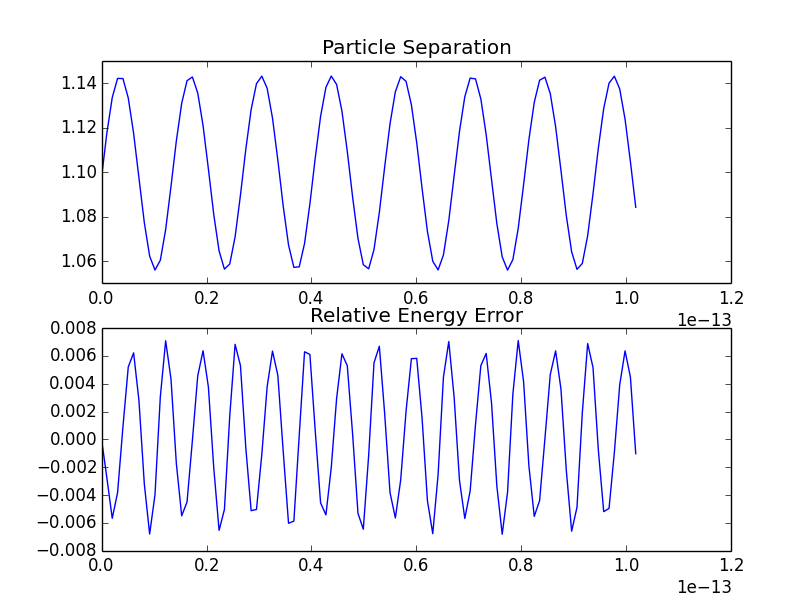
\includegraphics[width=\textwidth]{largedt}
			\caption*{$\Delta t = 0.1\times(10.8\text{fs})$}
		\end{subfigure}
		\begin{subfigure}{0.45\textwidth}
			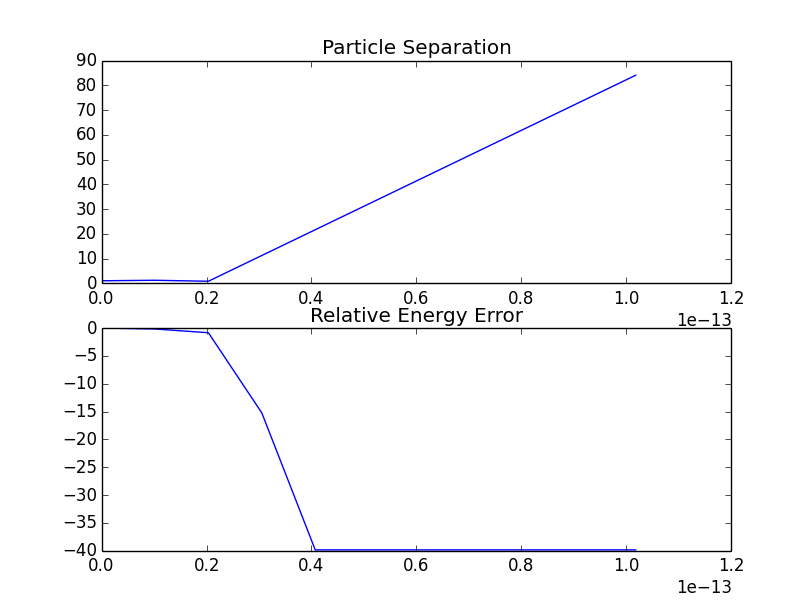
\includegraphics[width=\textwidth]{largerdt}
			\caption*{$\Delta t = 1\times(10.8\text{fs})$}
		\end{subfigure}
	\end{figure}
	
	The left figure is clearly showing signs of inaccuracy and is rather jagged. The right figure is wildly inaccurate.
	
	To determine the $dt_{\text{max}}$ we have to find the largest possible $dt$ such that the relative energy error has magnitude less than $10^{-3}$. This will be different for each integrator. For the velocity Verlet integrator we find that $dt_{\text{max}} \approx 0.1u $ For the symplectic Euler integrator we find that $dt_{\text{max}} \approx 0.015u,$ which is far smaller than the maximum timestep for the Verlet integrator. This shows that the Verlet integrator is more accurate with a larger timestep. 
	
When we run the Verlet integrator for a decent period of time with the timestep set to $dt_{\text{max}}$ we see that the oscillations are contained within a packet that itself oscillates. We can determine the frequency of operation using XMGrace. We determine the frequency of $N_2$ to be $ $, which is 
\end{document}
